\begin{figure}[h!]
    \centering
    \caption{Sample of ZIP codes in Zillow data vs.\ population density}
    \label{fig:map_zillow_sample}

    \begin{subfigure}{1\textwidth}
        \caption{Zillow ZIP codes}
        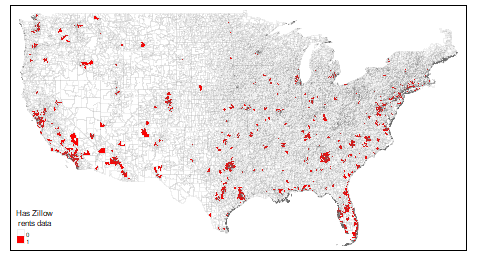
\includegraphics[width = 0.95\textwidth]
            {maps_US/output/USPS_zipcodes_zillow_data.png}
    \end{subfigure}\\
    \begin{subfigure}{1\textwidth}
        \caption{Population Density}
        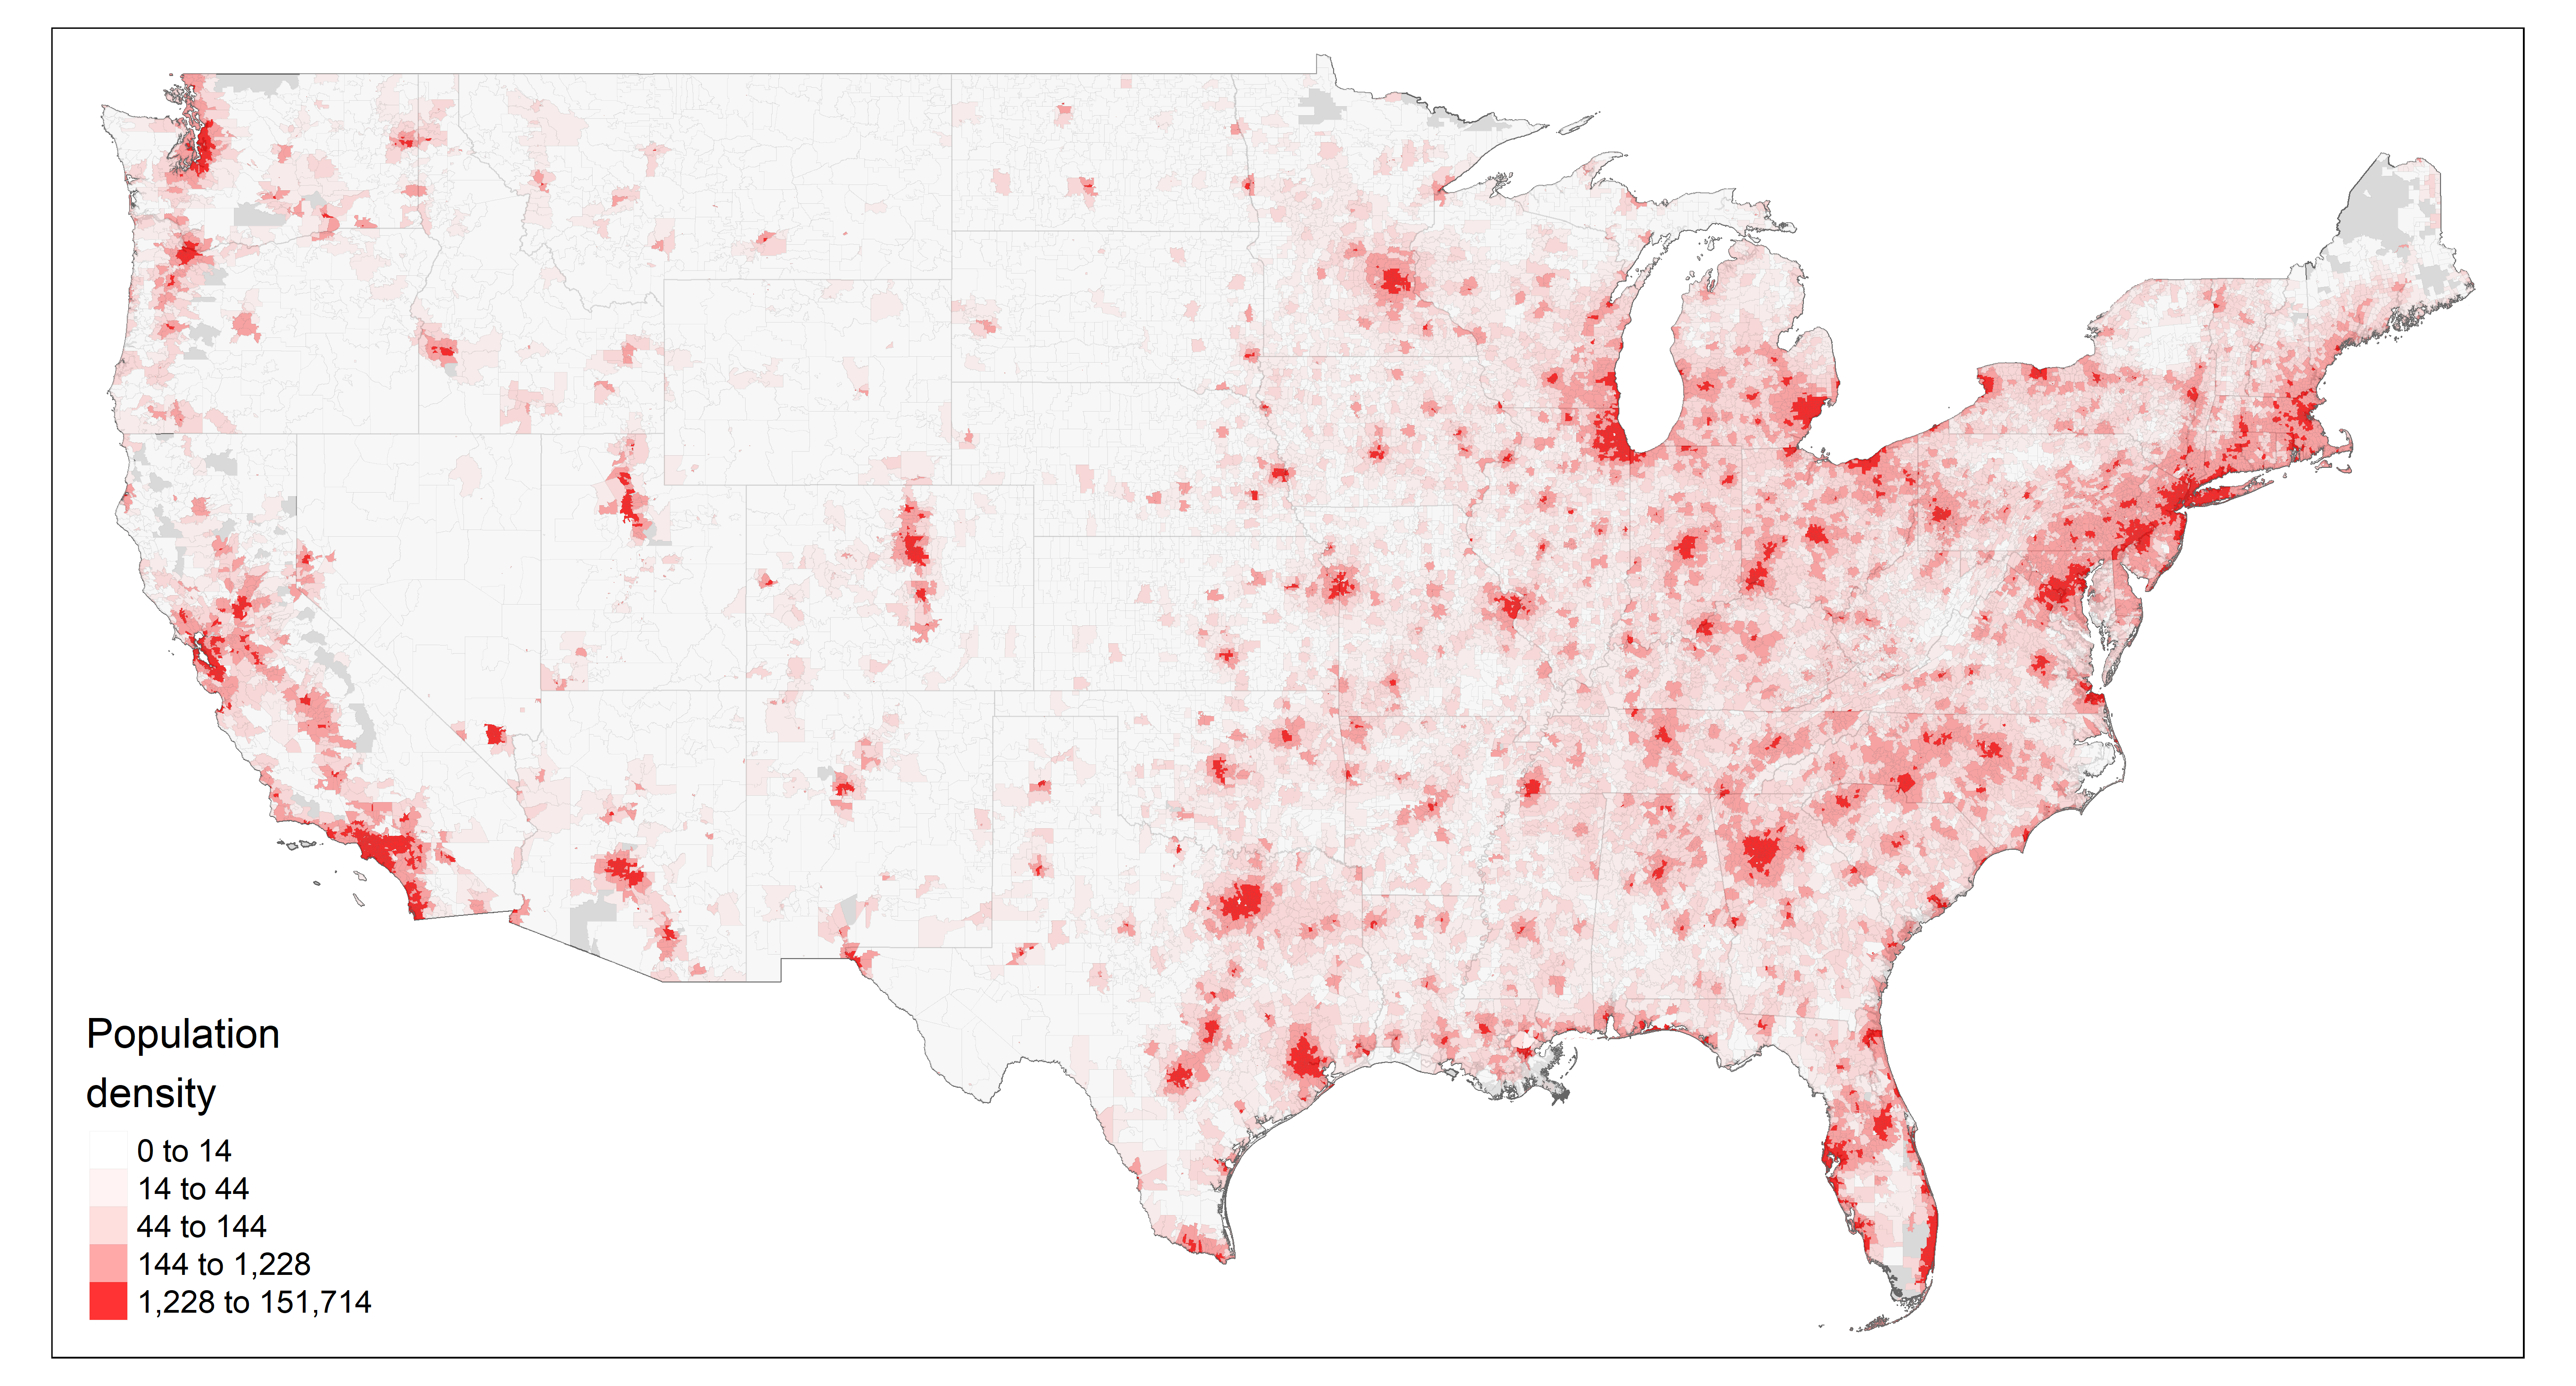
\includegraphics[width = 0.95\textwidth]
            {maps_US/output/USPS_zipcodes_pop_density.png}
    \end{subfigure}

    \begin{minipage}{.95\textwidth} \footnotesize
        \vspace{3mm}
        Notes:
        Data are from \textcite{ZillowData} and CENSO (YYYY).
        %%
        %% SH: Add cite of census data used in the map
        %%
        The figure compares the USPS ZIP codes available in Zillow to the 
        population density.
        Panel (a) shows the sample of the ZIP codes that have rents data in the 
        SFCC category at any point in the period 2010--2019.
        Panel (b) shows quintiles of population density, measured in people per
        square kilometer.
        %%
        %% SH: Is this the right unit of pop density?
        %%
        %%  Comments on map, after seeing it in PDF
        %%     Can we add the unit of pop density to the map?
        %%     Can we drop the box around the maps?
        %%     Can we make the white fill color coincide with the background white?
        %% 
    \end{minipage}
\end{figure}
